%Dovremmo forse aggiungere due parole sulle C* algebras: non sono stateintrodotte proprio per evitare il tensor product in infinitedimensional systems?
%%%%%%%%%%%%%%%%%%%%%%%%%%%%%%%%%%%%%%%%%%%%%%%%%%%%%%%%%%%%%%%%%%%%%%%%
% The four postulates of quantum mechanics are three
%%%%%%%%%%%%%%%%%%%%%%%%%%%%%%%%%%%%%%%%%%%%%%%%%%%%%%%%%%%%%%%%%%%%%%%%
\documentclass[aps,prl,amsmath,amssymb,twocolumn,nofootinbib]{revtex4}
%\documentclass[twocolumn,aps,showpacs,prl,groupedaddress]{revtex4}
%\usepackage{amssymb,stackengine}
\usepackage{amssymb}
\usepackage{color}
\usepackage{graphicx}
\usepackage{epsfig,amssymb,amsmath,amsthm}
%\usepackage[active]{srcltx}
%\usepackage[hypertex,linkcolor=red]{hyperref}

\usepackage{color}
\usepackage{cancel}
\usepackage{tikz-cd}

\theoremstyle{plain}
\newtheorem{thrm}{Theorem}[section]
\newtheorem{form}[thrm]{Formalization}
\newtheorem{prop}[thrm]{Proposition}
\newtheorem{lem}[thrm]{Lemma}

\theoremstyle{definition}
\newtheorem{defn}[thrm]{Definition}
\newtheorem{post}{Postulate}[]
\renewcommand*{\thepost}{(\alph{post})}

\theoremstyle{remark}
\newtheorem*{remark}{Remark}


\newcommand{\blue}{\color{blue}}  %NON LINEAR
\newcommand{\red}{\color{red}}
\newcommand{\cyan}{\color{cyan}}
\newcommand{\green}{\color{green}} %THEORY quantum state estimation
\newcommand{\yellow}{\color{yellow}} %THEORY quantum channel estimation

\DeclareMathOperator{\spn}{span}

\newcommand{\pj}[1] {\underbar{$#1$}}
%\newcommand{\pj}[1] {\overline{#1}}

\def\>{\rangle}
\def\<{\langle}
\def\ca{_{\cal A}}
\def\cb{_{\cal B}}
\def\cc{_{\cal C}}
%\def\comment#1{}
\def\comment#1{ [{\bf Comment Lor:} {\sf #1}]}
\def\commentg#1{ [{\bf Comment Gabriele:} {\sf #1}]}
\def\labell#1{\label{#1}}
%\def\labell#1{\label{#1}{\mbox{{\tiny #1}}}}
%\def\section#1{{\par\em #1:--- }}
\def\togli#1{}
\def\sh{\mbox{sh}}
\def\iden{\openone}
\begin{document}
	
	\fbox{{\scriptsize Internal report. \today}}\title{The four postulates of quantum mechanics are three}
	\author{Gabriele Carcassi$^1$, Lorenzo Maccone$^2$ and Christine A. Aidala$^1$
	}\affiliation{\vbox{1.~Physics Department, University of Michigan, 450 Church Street,
			Ann Arbor, MI 48109-1040,
			United States}\\
		\vbox{2.~Dip.~Fisica and INFN Sez.\ Pavia, University
			of Pavia, via Bassi 6, I-27100 Pavia, Italy}}
	\begin{abstract}
		The tensor product postulate of quantum mechanics states that the
		Hilbert space of a composite system is the tensor product of the
		components' Hilbert spaces. All current formalizations of quantum
		mechanics that do not contain this postulate contain some equivalent
		postulate or assumption (sometimes hidden). Here we give a natural
		definition of composite system as a set containing the component
		systems and show how one can logically derive the tensor product
		rule from the state postulate and from the measurement postulate. In
		other words, our paper reduces by one the number of postulates
		necessary to quantum mechanics.
	\end{abstract}
	\pacs{}
	% Measurement theory (quantum mechanics), 03.65.Ta Mechanics quantum,
	% 03.65.-w noise quantum, 42.50.Lc quantum information, 03.67.Ac
	% Quantum information, 03.67.-a Quantum fluctuations, 42.50.Lc quantum
	% mechanics, 03.65.Ta quantum optics, 42.50.Gy
	\maketitle
	
	
	The tensor product postulate does not appear in all axiomatizations of
	quantum mechanics: it has even been called ``postulate 0'' in some
	literature \cite{zurek}. A widespread belief is that it is a direct
	consequence of the superposition principle, and it is hence not a
	necessary axiom. {\em This belief is mistaken}: the superposition
	principle is encoded into the quantum axioms by requiring that the
	state space is a {\em linear} vector space. This is, by itself,
	insufficient to single out the tensor product, as other linear
	products of linear spaces exist, such as the direct product, the
	topological product or the direct sum of vector spaces, which are used
	in classical mechanics to combine state spaces of linear systems.
	This belief may have arisen from the seminal book of Dirac
	\cite{diracbook}, who introduces tensor products (Chap.~20) by
	appealing to linearity. However, he adds the seemingly innocuous
	request that the product among spaces be distributive (rather,
	bilinear), which is equivalent to postulating tensor products (or
	linear functions of them). This is not an innocuous request. For
	example it does not hold where the composite vector space of two
	linear spaces is described by the direct product, e.g.~in classical
	mechanics, for two strings of a guitar: it is not distributive.
	[General classical systems, not only linear ones, are also composed
	through the direct product.] Of course, Dirac is not constructing an axiomatic
	formulation, so his `sleight of hand' can be forgiven. In contrast, von
	Neumann (\cite{vonneumannbook} Chap.~VI.2, also \cite{jauch})
	introduces tensor products by noticing that this is a natural choice
	in the position representation of wave mechanics (where they were
	introduced in \cite{weyl,epr}), and then {\em explicitly postulates}
	them in general: ``This rule of transformation is correct in any case
	for the coordinate and momentum operators [...] and it conforms with
	the [observable axiom and its linearity principles], we therefore
	postulate them generally.''  \cite{vonneumannbook}.  More mathematical
	or conceptually-oriented modern formulations
	(e.g.~\cite{ozawa,masanes,nielsenchuang}) introduce this postulate explicitly.
	An interesting alternative is provided in
	\cite{ballentinebook,ballentinepaper}: after introducing tensor
	products, Ballentine verifies a posteriori that they give the correct
	laws of composition of probabilities. Similarly, Peres uses
	relativistic locality \cite{peres}. While these procedures seemingly
	bypass the need to postulate the tensor product, they do not guarantee
	that this is the {\em only} possible way of introducing composite
	systems in quantum mechanics. In the framework of quantum logic,
	tensor products arise from some additional conditions \cite{matolcsi}
	which (in contrast to what is done here) are not connected to the
	other postulates. A similar approach was followed in \cite{aerts}
	where tensor products were obtained by specifying some additional
	physical requirements. In quantum field theory one tends to avoid
	problems connected with tensor products of infinite dimensional spaces
	by focusing on algebraic commutation structures, e.g.~\cite{giddins}.
	In particular, the recent MIP*=RE result \cite{mipre} implies that, in
	infinite dimensions, the tensor product is strictly less
	computationally powerful than the commutation structures, emphasizing
	the difference among these two structures, at least for the
	infinite-dimensional case. We will consider the non-relativistic
	setting here.
	
	In this paper we derive the tensor product postulate (which, hence,
	loses its status of postulate) from two other postulates of quantum
	mechanics: the state postulate and the measurement postulate. We start
	from the natural definition of a composite system as the set of two
	(or more) quantum systems, in the sense that the composite system is
	made of system $A$ {\em and} (joined with) system $B$, namely a set
	whose elements are the two systems and nothing else. We will focus on
	kinematically-independent systems, namely no superselection rules or
	other restrictions to the state space are present: it is possible to
	prepare each subsystem of a composite system in a state that is
	independent of the other systems (preparation independence).  This is
	the only case in which the tensor product can be properly employed
	\cite{susskind,zanardi,zanardilloyd}: the Hilbert space of composite
	systems that have restrictions is {\em not} the tensor product of the
	component spaces, but a subspace of it (e.g.~the anti-symmetric
	subspace for fermions). Typically this is ignored in the literature,
	since the tensor product formalism is very convenient and is often
	used also in these cases. Moreover, in accordance with the measurement
	postulate, we require that the probability distribution of the
	measurement outcomes of one system is independent of the other systems' (statistical
	independence). As detailed below, statistical independence is not an
	additional requirement: it is already contained in the measurement
	postulate.
	
	From the above definition of composite system, it follows that there
	must be a map $M$ that connects the states of the subsystems to the
	states of the composite system. A quantum state is a ray in Hilbert
	space, namely a set of vectors. The map $M$ on states 
	corresponds to a map $m$ on vectors. We then show that preparation
	independence and statistical independence imply three conditions on
	the map $m$: (H1)~totality: the map is defined on all states of the
	subsystems; (H2)~bilinearity: the map is bilinear thanks to the
	fundamental theorem of projective geometry; (H3)~span surjectivity:
	the span of the image of map coincides with the full composite Hilbert space.
	We then prove that, if these three conditions H1, H2 and H3 hold, then
	the map $m$ is the tensor product, namely the Hilbert space of the
	composite system is a tensor product of the components: the tensor
	product ``postulate'', which hence loses its status of a postulate. An
	overview of all these logical implications is given in
	Fig.~\ref{f:fig}. The rest of the paper contains the sketch of this
	argument. Refer to the supplementary material for a more rigorous proof of the \emph{same} argument.
	
	\begin{figure}[h]
		\includegraphics[width=\linewidth, trim={0.2in 5.2in 2.5in 0.6in}, clip=true]{fig.eps}
		\caption{Schematic depiction of the logical implications used here. FTPG stands for ``Fundamental Theorem of Projective Geometry''
			\label{f:fig}}\end{figure}
	\togli{
		\begin{widetext}\begin{verbatim}
			* P1: states and observable postulate.
			* P2: Born rule (measurement postulate). 
			* P1 -> systems can be prepared unconditionally in any state.
			* P2 -> the outcome probabilities depend only on the scalar
			product.
			* 2. Def: Composite system definition: A composite system is a collection of
			(all compatible state give a 
			preparation) and only of (all composite preparations give non-trivial
			measurement on subsystems) the subsystems 
			* P1+ Def -> 1. Preparation independence (all state pairs are compatible)
			* P2+ Def -> 3. Span surjectivity (I.4=H3) (all C is spanned by AxB) 
			* 3 -> 6. Basis carries over I.7
			* 1 + 2 -> 4. Injectivity (M total function) I.5=H1
			* 2 + PI -> 5. Statistical independence I.6 (probability on compatible
			pairs where one subsystem does not change) 
			* 5 -> 7. I.8=H2: scalar product carries over (fundamental theorem of
			projective geometry).
			* 7 + 6 + 4 (i.e. H1+H2+H3) -> 8. m is tensor product   
			\end{verbatim}\end{widetext}
	}
	
	We start by noting that the tensor product is uniquely
	characterized, up to isomorphism, by a universal property regarding
	bilinear maps: given two vector spaces $\cal A$ and $\cal B$, the
	tensor product ${\cal A}\otimes{\cal B}$ and the associated bilinear
	map $T : \cal A \times \cal B \to {\cal A}\otimes{\cal B}$ have the property
	than any bilinear map $m:{\cal A}\times{\cal B}\to{\cal C}$ factors
	through $T$ uniquely.  This means that there exists a {\em unique}
	$\hat m$, dependent on $m$, such that $\hat m \circ T=m$.  In other
	words, the following diagram commutes:
	\begin{center}
		\begin{tikzcd}\mathcal{A}\times\mathcal{B} \arrow[rd, "m"]\arrow[r, "T"] & \mathcal{A}\otimes\mathcal{B}\arrow[d, "\hat{m}"] \\
			& \mathcal{C}
		\end{tikzcd}
	\end{center}
	
	We use the axiomatization of quantum mechanics based on the following
	postulates (e.g.~\cite{ozawa,nielsenchuang}): (a)~The state of a
	system is described by a ray $\pj{\psi}$ corresponding to a set of
	non-zero vectors $|\psi\>$ in a complex Hilbert space, and the
	system's observable properties are described by self-adjoint operators
	acting on that space; (b)~The probability that a measurement of a
	property $X$, described by the operator with spectral decomposition
	$\sum_{x,i}x|x_i\>\<x_i|$ ($i$ a degeneracy index), returns a value
	$x$ given that the system is in state $\pj{\psi}$ is
	$p(x|\psi)=\sum_i|\<\psi|x_i\>|^2$ (Born rule). (c)~The state
	space of a composite system is given by the tensor product of the
	spaces of the component systems; (d)~The time evolution of an isolated
	system is described by a unitary operator acting on a vector
	representing the system state, $|\psi({t})\>=U_{t}|\psi({t}=0)\>$ or,
	equivalently, by the Schr\"odinger equation. The rest of quantum
	theory can be derived from these axioms. While some axiomatizations
	introduce further postulates, we will be using only (a) and (b) to
	derive (c), so the above are sufficient for our aims.
	
	\togli{This axiomatization implicitly contains a definition of ``quantum
		system'' which is crucial for what follows, so we need to clarify the
		assumptions that it contains. We will use the following definition for
		a quantum system\togli{$\stackon[1pt]={\mbox{\tiny
					def}}$}$\stackrel{\mbox{\tiny def}}=${\em ``a quantum degree of
			freedom with $d$ (possibly discrete, or continuous, infinite)
			mutually exclusive (commuting) values for each of its properties.
			Its mathematical description is through a Hilbert space of dimension
			$d$ which contains all the states that describe the values of its
			possible properties. In accordance with the postulate (a), these
			values correspond to a basis of the space, given by the eigenvectors
			of the observable corresponding to that property''}. \commentg{We may have to revise to be more clear. Where is this used?} }
	As stated
	above, we will limit ourselves to kinematically-independent systems,
	where all state vectors $|\psi\>$ in the system's Hilbert space $\cal H$
	describe a valid state, {\em unconditioned on anything else}. In
	particular, we note that restrictions due to superselection rules
	arise either from practical (not fundamental) limitations on the
	actions of the experimenter \cite{susskind,zanardi,zanardilloyd} or
	from the use of ill-defined quantum systems. For example, in
	situations where indistinguishability plays a role (e.g.~in QFT), one
	cannot consider an electron as a quantum system: in this case the
	quantum system is the field. The electron is an excitation of the
	field, {\em not} a (sub)system.
	
	This implies that the ``system'' is kinematically independent from
	anything else.  We call this condition ``preparation independence''.
	[We emphasize that the kinematic independence is inequivalent to
	dynamical independence (or isolation).  Indeed if two systems
	interact, their interaction may lead to dynamical restrictions in the
	state spaces. We will not consider dynamical evolution in this paper,
	which is contained in postulate (d).]
	
	The definition of a composite system as containing {\em only} the
	collection of the subsystems means that any preparation of both
	subsystems independently must correspond to the preparation of the
	composite system. Since states are defined by postulate (a) as rays in
	the respective Hilbert spaces, there must exist a map $M : \pj{\cal A}
	\times \pj{\cal B } \to \pj{\cal C}$ that takes a pair of states for
	the subsystems ($\pj{\cal A}$ and $\pj{\cal B }$ represent the
	projective spaces and the Cartesian product is the set of all possible
	pairs) and returns a state in the projective space $\pj{\cal C}$ for
	the composite. The map $M$ that acts on rays corresponds to a map $m:{\cal A}\times{\cal B}\to{\cal C}$ that
	acts on vectors in the Hilbert spaces $\cal A$, $\cal B$ and $\cal C$.
	Namely, $\pj{m(a,b)}=M(\pj{a},\pj{b})$ where the underline sign
	indicates the elements in the projective space. We will prove that the
	map $m$ is the tensor product.
	
	The map $M$ must be injective: as said above, different states of the
	subsystems must correspond, by definition of composite system, to
	different states of the composite. Moreover, preparation independence
	implies that $M$, and hence $m$, must be total maps: each subsystem of
	the composite system can be independently prepared and gives rise to a
	state of the composite (condition H1).  H1 is not sufficient
	to identify the tensor product: by itself it does not even guarantee
	that the map $m$ is linear.
	
	Postulate (b) contains the connection between quantum mechanics
	and probability theory. It must then implicitly contain the
	axiomatization of probability, e.g.~see
	\cite{ballentinepaper,ballentinebook,cox}. One of the axioms of
	probability theory (axiom 4 in \cite{ballentinepaper}) asserts that
	the joint probability of events $a$ and $b$ given $z$ is
	$p(a\wedge b|z)=p(a|z)\:p(b|z\wedge a)$. Then the events $a$ and $b$ are
	independent given $z$ if and only if $p(a\wedge b|z)=p(a|z)\:p(b|z)$ (this
	is the {\em definition} of independent events). Since the Born
	probability formula in postulate (b) contains only quantities of the
	system (the state and the observable's eigenstates {\em of the
		system}), it implies the ``statistical independence'' between
	different systems if they are prepared independently. Namely, the
	outcome probability of one is independent of any properties of any
	other in the absence of any dynamical coupling and supposing
	independent preparation. [Of course, the dynamics may couple the state
	of the system to other systems so that the outcomes may depend on what
	happens to other systems.  Analogously, one may prepare the system in
	a way that depends on other systems. But we consider independent
	preparations and do not consider dynamics, as it is sufficient for our
	aims.] We can then formalize ``statistical independence'' of
	independently prepared systems by saying that their Born rule
	satisfies:
	\begin{eqnarray}
	p(a\wedge b|\psi_{\cal A}\wedge \psi_{\cal B})&=&p(a|\psi_{\cal A}\wedge \psi_{\cal
		B})\:p(b|\psi_{\cal A}\wedge \psi_{\cal B})\nonumber\\&=& p(a|\psi_{\cal
		A})\:p(b|\psi_{\cal B})
	\labell{bindip}\;,
	\end{eqnarray}
	where $\psi_{\cal A}$, $\psi_{\cal B}$ represent the independent
	preparations of the states of the systems $\cal A$, $\cal B$ and $a$,
	$b$ the measurement outcomes of two observables on $\cal A$ and $\cal
	B$ respectively. The first equality in \eqref{bindip} embodies the
	definition of statistical independence, the second follows from the
	form of the Born rule for independently prepared systems (the
	probability depends only on the state and observables of each system
	on its own).
	
	A particular case is when one system is
	prepared in a fixed eigenstate $|b\>$ of the observable measured on it,
	$p(a\wedge b|\psi\wedge b)=p(a|\psi)\:p(b|b)=p(a|\psi)$, where the last equality follows from the Born rule since $\<b|b\>=1$. 
	If we define $M_b(\pj{a}) = M(\pj{a},\pj{b})$, substituting the values of the
	probabilities from the Born rule, we have:
	\begin{align} &\Big|\Big\<M\left(\pj{a},\pj{b}\right)\Big|M\left(\pj{\psi},\pj{b}\right)\Big\>_{\cal C}\Big|^2
	=\Big|\Big\<M_b\left(\pj{a}\right)\Big|M_b\left(\pj{\psi}\right)\Big\>_{\cal C}\Big|^2
	\nonumber \\&
	=\left|\<a|\psi\>_{\cal A}\right|^2
	\labell{questa},
	\end{align}
	where the first and second terms contain the scalar product in the composite
	space $\cal C$. [This is not a new assumption: it follows from the
	measurement postulate (b) for the composite system.] This means that,
	when one subsystem is prepared in an eigenstate of what is measured
	there, the state space of the other is mapped preserving the square of
	the inner product.
	
	Since the square of the inner product is preserved, orthogonality and
	the hierarchy of subspaces are preserved through $M_b$, making $M_b$ a
	colinear transformation by definition. In this case, the fundamental
	theorem of projective geometry \cite{fun} applies, which tells us that
	a unique semi-linear map $m_b$ that acts on the vectors exists in accordance with $M_b$.
	Moreover, conservation of probability further constrains it to be
	either linear or antilinear. This tells us that the corresponding $m$
	is either linear or antilinear in the first argument. Namely, if
	\eqref{questa} holds, then
	\begin{align}
	\<a|\psi\>=\<m(a,b)|m(\psi,b)\>\labell{h2}\;
	\\\mbox{ or }
	\<a|\psi\>=\<m(\psi,b)|m(a,b)\> \labell{h2b}.
	\end{align}
	We can ignore the antilinear case \eqref{h2b}, which simply
	corresponds to the map $m$ mapping kets of one or both subsystems into
	bras before outputting the composite system (all these maps are
	trivially physically equivalent, since the dual-space description of a
	quantum system through bras is equivalent to the description using
	kets). We can now repeat the same analysis for the second argument of
	$m$ to conclude that it is a bilinear map, condition (H2).
	
	The last condition (H3) follows directly from the definition of a
	composite system. Since it is composed {\em only} of the component
	systems, for any state $c$ of the composite system, we must find at least one pair $(a, b)$ such that $p(a\wedge b | c)\neq 0$. It follows that the map $m$ is span-surjective: namely the
	span of the map applied to all states in the component systems spans
	the composite system state space. In other words, the composite does
	not contain states that are totally independent of (i.e.~orthogonal
	to) the states of the components.
	
	We have obtained the conditions H1, H2 and H3 from the state postulate
	(a), the measurement postulate (b) and the definition of composite
	systems. We now prove that these three conditions imply that the (up
	to now unspecified) composition rule $m$ is the tensor product. More
	precisely, given a total, span-surjective, bilinear map $m:{\cal A}\times{\cal B}\to{\cal C}$ that preserves the square of the inner
	product, we find that $\cal C $ is equivalent to
	$\cal A \otimes \cal B $ and that $m=\otimes$.
	
	Proof. Step 1: the bases of the component systems are mapped to a
	basis of the composite system. Because of totality property (H1) and
	because the square of the inner product is preserved, we can conclude
	that, given two orthonormal bases $\{|a_i\>\}\in{\cal A}$ and
	$\{|b_j\>\}\in{\cal B}$,
	$|\<m(a_i,b_j)|m(a_k,b_\ell)\>|^2=\delta_{ik}\delta_{j\ell}$, namely
	$\{|m(a_i,b_j)\>\}$ is an orthonormal set in $\cal C$.  Moreover, the
	surjectivity property (H3) guarantees that in $\cal C$ no vectors are
	orthogonal to this set. This implies that it is a basis for $\cal C$.
	
	Step 2: Since $m : \mathcal{A} \times \mathcal{B} \to \mathcal{C}$ is
	a bilinear operator (property H2), thanks to the universal property of
	the tensor product we can find a unique linear operator $\hat{m} :
	\mathcal{A} \otimes \mathcal{B} \to \mathcal{C}$ such that $m(a, b) =
	\hat m(a \otimes b)$. The set $\{ \hat m(a_i\otimes b_j)$ with
	$|a_i\>$ and $|b_j\>$ orthonormal bases for $\cal A$ and ${\cal B}\}$
	forms a basis for $\cal C$, since $\hat m(a_i\otimes b_j)=m(a_i,b_j)$
	and we have shown above that the latter is a basis.  Thus,
	\begin{align} 
	&\<\hat m(a_i\otimes b_j)|\hat m(a_k\otimes b_\ell)
	\>_{\mathcal{C}}=\<m(a_i,
	b_j)|m(a_k,b_\ell)\>_\mathcal{C} \nonumber\\& =
	\delta_{ik}\delta_{j\ell}
	= \<a_i\otimes
	b_j| a_k \otimes b_\ell\>_{\otimes},
	\labell{ecco}\; 
	\end{align}
	where we used the orthonormality of the bases and the fact that
	$|a_i\otimes b_j\>$ is a basis of the tensor product space ${\cal
		A}\otimes{\cal B}$. The function $\hat{m}$, then, is an isomorphism
	over all elements of the basis $|a_i\otimes b_j\>$. It is then an
	isomorphism between $\cal C$ and ${\cal A}\otimes{\cal B}$. Namely,
	$|m(a_i,b_j)\>_{\cal C} = |\hat{m}(a_i\otimes b_j)\>_{\cal C} \cong
	|a_i\otimes b_j\>_\otimes$, where the first two vectors (in $\cal C$)
	are isomorphic to the last vector (in the tensor product space ${\cal
		A}\otimes{\cal B}$). Namely, $\hat{m}$ maps bijectively to the
	tensor product, which implies the isomorphism ${\cal C}\cong{\cal
		A}\otimes{\cal B}$, i.e.~their equivalence through the map
	$\hat{m}$. Moreover, since ${\cal C}\cong{\cal A}\otimes{\cal B}$,
	then the map $m : \cal A \times \cal B \to \cal C$ is equivalent to
	the map $\otimes : \cal A \times \cal B \to \cal A \otimes \cal B$,
	i.e.~the maps $m$ and $\otimes$ are also equivalent through $\hat
	m$.$\square$
	
	\vskip 1\baselineskip A few comments on the proof: it is based on the
	universal property of the tensor product, which uniquely characterizes
	it. In Step 1 we showed that the bilinear map $m$ maps subsystems'
	bases into the composite system basis. We also know that there exists a
	tensor product map $ {T}=\otimes$ that can compose the vectors in $\cal A$
	and $\cal B$. In Step 2 we use the universal property: since $m$ is a
	bilinear map, we are assured that there exists a unique $\hat m$ such
	that $\hat m \circ T=m$. Since we show that $\hat m$ is an
	isomorphism, then $\hat{m}$ bijectively maps vectors in $\cal C$
	onto vectors in the tensor product space. Namely $m={T}=\otimes$.
	
	We conclude with some general comments. The tensor product structure
	of quantum systems is not absolute, but depends on the observables
	that are accessible \cite{zanardi,zanardilloyd}. This is due to the
	fact that an agent that has access to a set of observables will define
	quantum systems differently from an agent that has access to a
	different set of observables. Where one agent sees a single system, an
	agent that has access to less refined observables (and is then limited
	by some superselection rules) can consider the same system as composed
	of multiple subsystems. A typical example \cite{tellerbook} comes from
	quantum field theory. It is customary in basically all quantum optics
	literature to treat different modes of the radiation field (e.g.~the
	output of two lasers) as independent systems composed through the
	tensor product.  Clearly the electromagnetic field is a single system
	and an agent who is able to access an optical mode that is a linear
	combination of the two will give a quantum description for it that
	cannot easily accommodate tensor products. Similarly, an agent can
	consider two electrons as two systems, joined with the tensor product,
	whenever they are distinguishable for all practical purposes (e.g.~the
	electrons are in widely separated physical locations). Yet, in
	principle, electrons are just excitations of a field, and the `true'
	quantum system is the field, not the single electrons
	\cite{teller,tellerbook}.  So, in quantum field theory, the quantum
	systems that should be joined through tensor products are the
	different fields and {\em not} the particles, which are just
	excitations (states) of the fields. In the words of Teller
	(\cite{tellerbook}, pg.22), tensor products can be safely used only if
	there is a ``primitive thisness'', which is captured in the definition
	of system.\togli{\comment{forse e' da spiegare meglio}}
	
	
	
	
	\togli{\comment{Commento finale da aggiungere?  E' interessante perche' tutto
			cio' ci dice che non otteniamo necessariamente il prodotto tensore,
			ma il prodotto tensore modulo una fase locale che e' fisicamente
			irrilevante. Viene da chiedersi se c'e' una qualche notazione
			(evidentemente piu' generale di quella di Dirac) che ci permetta di
			eliminare questa ambiguita' fisicamente irrilevante... La notazione
			di Dirac gia' elimina la necessita' di avere una rappresentazione
			per descrivere gli stati. Pero' evidentemente non elimina del tutto
			la ambiguita' di rappresentazione perche' un cambio di coordinate
			sia sugli stati che sugli operatori mi lascia invariata la fisica,
			ma non lascia invariata la notazione di Dirac...  Probabilmente la
			notazione che elimina l'ambiguita' e' quella che utilizza le matrici
			densita' invece dei vettori di stato (vedi Ozawa \cite{ozawa} e
			Holevo): le matrici densita' normalizzate sono phase-independent:
			$\rho=|\psi\>\<\psi|$. Attenzione: l'interpretazione di una matrice
			mista $\rho=\sum_ip_i|\psi_i\>\<\psi_i|$ come ``il sistema e' nello
			stato $|\psi_i\>$ con probabilita' $p_i$'' e' una CONSEGUENZA della
			regola di Born, quindi nella formalizzazione del postulato degli
			stati in termini di matrici densita', questa interpretazione non
			puo' apparire perche' e' una conseguenza di un altro postulato.}}
	
	It has been pointed out before that the quantum postulates are
	redundant: in \cite{masanes} it was shown that the measurement
	postulate (b) can be derived from the others (a), (c), (d). Here
	instead we have shown how the tensor product postulate can be
	logically derived from the state postulate (a), the measurement
	postulate (b) and a reasonable definition of independent systems, and
	we have described the logical relations among them.  Of course, we do
	not claim that this is the {\em only} way to obtain the tensor product
	postulate from the others.
	
	L.M. acknowledges useful discussions with M.~Ozawa, P.~Zanardi,
	S.~Lloyd, D.~Zeh, G.~Auletta, A.~Aldeni. We acknowledge funding from
	the Attract project through the Eu Horizon 2020 research and
	innovation programme under grant agreement No 777222.
	\begin{references}
		\bibitem{zurek} W.H. Zurek, Quantum Darwinism, Nature Phys. {\bf 5},
		181 (2009).
		\bibitem{diracbook}P.A.M. Dirac, The principles of quantum mechanics,
		(Clarendon Press, Oxford, 1966).
		\bibitem{vonneumannbook}J. von Neumann, Mathematical Foundations of
		Quantum Mechanics (Princeton Univ.  Press, 1955).
		\bibitem{jauch}J.M. Jauch, Foundations of quantum mechanics
		(Addison-Welsey, 1968), pg.~176.
		\bibitem{weyl} H. Weyl, Gruppentheorie und Quantenmechanik (Hirzel,
		Leipzig, 1928); translated by H. P. Robertson, The Theory of Groups
		and Quantum Mechanics (Methuen, London, 1931); reprinted by Dover,
		p. 91.
		\bibitem{epr}A. Einstein, B. Podolsky, N. Rosen, Can
		quantum-mechanical description of physical reality be considered
		complete?, Phys. Rev. {\bf 47}, 777 (1935).
		\bibitem{ozawa}M. Ozawa, {Uncertainty relations for noise and
			disturbance in generalized quantum measurements}, Ann. Phys.  {\bf
			311}, 350 (2004).
		\bibitem{masanes}L. Masanes, T.D. Galley, M.P. M\" uller, The
		measurement postulates of quantum mechanics are operationally
		redundant, Nat. Commun. {\bf 10}, 1361 (2019).
		\bibitem{nielsenchuang}M. A. Nielsen and I. L. Chuang, Quantum Computation
		and Quantum Information (Cambridge University Press, Cambridge,
		2000).
		\bibitem{ballentinebook}L.E. Ballentine, Quantum Mechanics, a modern
		development (World Scientific, 2014).
		\bibitem{ballentinepaper}L.E. Ballentine, Probability theory in
		quantum mechanics, Am. J. Phys. {\bf 54}, 883 (1986).
		\bibitem{cox}R.T. Cox, The Algebra of Probable Inference (J. Hopkins
		press, 1961).
		\bibitem{peres}A.~Peres, Classical interventions in quantum systems.
		II. Relativistic invariance, Phys. Rev. A {\bf 61}, 022117 (2000).
		\bibitem{matolcsi} T. Matolcsi, Tensor product of Hilbert lattices and
		free orthodistributive product of orthomodular lattices, Acta Sci.
		Math. (Szeged), {\bf 37}, 263 (1975).
		\bibitem{aerts} D. Aerts, I. Daubechies, Physical justification for
		using the tensor product to describe two quantum systems as one
		joint system, Helv. Phys. Acta {\bf 51}, 661 (1979).
		\bibitem{giddins}S.B.~Giddings, Hilbert space structure in quantum
		gravity: an algebraic perspective. J. High Energ. Phys. 2015, 1
		(2015).% https://doi.org/10.1007/JHEP12(2015)099
		\bibitem{susskind}Y. Aharonov, L. Susskind, Charge superselection
		rule, Phys. Rev. {\bf 155}, 1428 (1967).
		\bibitem{zanardi}P. Zanardi, Virtual Quantum Subsystems, Phys. Rev.
		Lett {\bf 87}, 077901 (2001).
		\bibitem{zanardilloyd} P. Zanardi, D.A. Lidar, S. Lloyd, Quantum
		Tensor Product Structures are Observable Induced, Phys. Rev. Lett.
		{\bf 92},060402 (2004).
		\bibitem{tellerbook}P. Teller, An Interpretive Introduction to Quantum
		Field Theory (Princeton Univ. Press, 1997).  
		\bibitem{teller}M. Redhead, P. Teller, Particles, Particle Labels, and
		Quanta: The Toll of Unacknowledged Metaphysics, Found. Phys. {\bf
			21}, 43 (1991).
		\bibitem{mipre}Z. Ji, A. Natarajan, T. Vidick, J. Wright, H. Yuen, MIP*=RE, arXiv:2001.04383 (2020). %https://quantumfrontiers.com/2020/03/01/the-shape-of-mip-re/
		\bibitem{fun} E. Artin: Geometric algebra, Interscience Publishers Inc (1957)
		\bibitem{holevo}A. Holevo, Probabilistic and statistical aspects of
		quantum theory, (North Holland, 1982).
	\end{references}
	
	\vskip 5\baselineskip
	
	\section{Appendix: mathematical formulation}\label{app}
	\setcounter{section}{1}
	
	The following section needs to distinguish the projective space from
	the Hilbert space itself. As this is seldom done in quantum mechanics,
	we review some concepts in that context and introduce the notation
	that we will be using. If $X$ is a Hilbert space, we denote $\pj{X}$
	the projective space. The projective space is mathematically
	constructed from the Hilbert space by removing the origin and
	quotienting by the equivalence relationship $v \sim \lambda v$, $v\in
	X$ and $\lambda\in\mathbb{C}$. A quantum state is a point in
	projective space. Each point of the projective space is called a ray,
	because for a real vector space to would correspond to a line going through
	the origin, with the origin removed. As we are in a complex space, the
	ray should be thought as a complex plane without the origin, which is
	the space of the vectors reachable from a fixed one through
	multiplication by a complex number. It can also be thought as a
	subspace of dimension one.
	
	Given a vector $v \in X$, we will denote $\pj{v}$ the ray in the
	projective space corresponding to $v$. Note that $\pj{v}$ denotes a
	quantum state, without having picked a modulus or phase. Given two or
	more vectors $v_1, ..., v_n \in X$, the subspace of $X$ they span
	(i.e.~all the vectors reached by linear combinations) is noted by
	$Sp(v_1, ..., v_n)$. Note that this subspace will correspond to a set
	of rays in the projective space, which we note as $\pj{Sp(v_1, ...,
		v_n)}$. Given $v,w \in X$, we can write $P(v|w) = \frac{|\< v | w
		\>|^2}{\< v | v \>\< w | w \>}$ which corresponds to the probability
	of observing $v$ given $w$ was prepared. Note that $P(v|w) = P(\lambda
	v| \mu w)$, with non-null $\lambda,\mu\in{\mathbb C}$, and therefore
	one can write $P(\pj{v} | \pj{w})\equiv P(v|w)$ as a function of the
	rays.
	
	
	\begin{post}\label{post_state}
		The state of a quantum system is described by a ray $\pj{\psi} = \{
		\alpha |\psi\> \, |$ non-null $\alpha \in
		\mathbb{C},|\psi\>\in\mathcal{H}\}$ in a complex Hilbert space
		$\mathcal{H}$, and the system's observable properties are described
		by self-adjoint operators acting on that space. %All vectors represent possible   system system states and all self-adjoint operators represent possible system   observables.
	\end{post}
	
	\begin{remark}
		All proofs, except one, should not depend on the dimensionality of
		the space. The exception is proposition \ref{prop_fundProj} which
		works if the basis for the space is finite since we are constructing
		the map one component at a time. It should be possible to extend it
		using weak convergence in the case of countable basis
		(i.e. separable Hilbert spaces) by creating a sequence that
		converges to each vector. We are not specifically addressing this
		case in this paper.
	\end{remark}
	
	\begin{post}\label{post_measurements}
		The probability that a measurement of a property $X$, described by the operator with
		spectral decomposition $X = \sum_{x,i }x \frac{| x_i \> \< x_i |}{\< x_i | x_i \>}$  where $i$ is a degeneracy index, returns a value $x$ depends only on $X$ and on the state of the system $\pj{\psi}$ and is given by $P(x|\pj{\psi})=\sum_i \frac{\<\psi| x_i \> \< x_i |\psi\>}{\< \psi | \psi \>\< x_i | x_i \>}$
		(Born rule).\end{post}
	
	
	\begin{defn}[Compatible states]\label{def_compatible}
		Let A and B be two systems. Let ${\mathcal{A}}$ and ${\mathcal{B}}$
		be their corresponding state spaces. We say two (pure) states $(\pj{a},
		\pj{b}) \in \pj{\mathcal{A}} \times \pj{\mathcal{B}}$ are compatible
		iff the respective systems can be prepared in such states at the
		same time. Formally, the proposition $\pj{a} \wedge \pj{b}$ is
		possible, which means it does not correspond to the empty set in the
		$\sigma$-algebra of the probability space\footnote{The impossible event is not an event with probability zero, rather it is an event that cannot be created at all. For example, ``the dice shows a number that is even and less than two'', or ``the electron is prepared in spin up along $x$ and also along $z$'' are impossible events.}.
	\end{defn}
	
	{Note that the proposition $\pj{a} \wedge \pj{b}$ refers to either
		preparation or measurement of both systems  in the respective state.
		The proposition $\pj{a} | \pj{b}$, instead, is the one that
		corresponds to preparing one system in one state and measuring the
		other system in the other state \cite{cox}. Incompatible states
		refer to non-commuting observables.}
	
	\begin{defn}[Preparation independence]\label{def_indep}
		Two systems are said independent iff the preparation of one does not affect the preparation of the other. Formally, all (pure) state pairs $(\pj{a}, \pj{b}) \in \pj{\mathcal{A}}\times \pj{\mathcal{B}}$ are compatible.
	\end{defn}
	
	\begin{prop}\label{prop_singleBorn}
		Given two systems, each prepared independently in their own state, the probability of measuring a value for one system depends only on the preparation of that system. That is, $P(\pj{a_1}|\pj{a_2}\wedge \pj{b})=P(\pj{a_1}|\pj{a_2})$.
	\end{prop}
	\begin{proof}
		We first note that, by postulate \ref{post_measurements}, the probability of measuring a value for one system depends only on the preparation of that system, which means that it is independent of the properties of any other system. Therefore $P(\pj{a_1} | \pj{a_2} \wedge \pj{b}) = \frac{\<a_1| a_2 \> \< a_2 |a_1\>}{\< a_1 | a_1 \>\< a_2 | a_2 \>} = P(\pj{a_1} | \pj{a_2})$
	\end{proof}
	
	\begin{defn}[Composite systems]\label{def_comp}
		Let A and B be two systems. The composite system C of A and B is formed by the simple collection of those and only those two systems, in the sense that it satisfies the following two requirements.
		\begin{enumerate}
			\item Every preparation of both subsystems is a preparation of the
			composite. Formally, let $\pj{\mathcal{C}}$ be the state space
			for C, there exists a map (not yet specified)
			$M:\pj{\mathcal{A}}\times\pj{\mathcal{B}}\to\pj{\mathcal{C}}$
			such that, for any compatible pair of (pure) states $(\pj{a},\pj{b}) \in \pj{\mathcal{A}}\times\pj{\mathcal{B}}$, the proposition $\pj{a} \wedge \pj{b}$ is equivalent to the (pure) state $M(\pj{a},\pj{b}) \in \pj{\mathcal{C}}$ where $M$ returns the state of the composite system where the subsystems were prepared in the given states. In other words, $\pj{a} \wedge \pj{b}$ and $M(\pj{a},\pj{b})$ correspond to the same event in probability space\footnote{We will end up proving that the map $M$ leads to the tensor product.}.
			\item Every preparation of the composite gives a non-trivial measurement on the components. Formally, for every $\pj{c} \in \pj{\mathcal{C}}$, we can find at least $\pj{a} \in \pj{\mathcal{A}}$ and $\pj{b} \in \pj{\mathcal{B}}$ such that $P(\pj{a} \wedge \pj{b}|\pj{c})\neq 0$. 
		\end{enumerate}
		Requirement 1 ensures that the composite system contains all the properties of the components. Requirement 2 ensures that it does not contain properties that are orthogonal to all the components' properties, i.e.~that the composite system contains {\em only} the components.
	\end{defn}
	
	\begin{prop}[Span surjectivity, H3]\label{prop_spanSurj}
		The map $M :
		\pj{\mathcal{A}}\times\pj{\mathcal{B}} \to \pj{\mathcal{C}}$ is span
		surjective, meaning that the span of the image coincides with the
		whole space. That is $Sp(\{ c \in \mathcal{C} \, | \, \pj{c} \in
		M(\pj{\mathcal{A}}, \pj{\mathcal{B}})\}) = \mathcal{C}$.
	\end{prop}
	\begin{proof}
		Consider $I=\{ c \in \mathcal{C} \, | \, \pj{c} \in M(\pj{\mathcal{A}}, \pj{\mathcal{B}})\}$ and its span. This forms a subspace of $\mathcal{C}$. By requirement 2 of \ref{def_comp}, for any $c \in \mathcal{C}$ we can always find $a \in \mathcal{A}$ and $b \in \mathcal{B}$ such that $P(\pj{a} \wedge \pj{b} | \pj{c} )\neq 0$. This means there is no element in $\mathcal{C}$ that is orthogonal to $Sp(I)$, therefore $Sp(I)$ must cover the whole $\mathcal{C}$.
	\end{proof}
	
	\begin{prop}[Totality, H1]\label{prop_totality}
		The map $M$ is in general a partial function.\footnote{A partial
			function is one that is not defined on the full domain. For
			example, $\sqrt(x)$ is a partial function since is not defined for
			$x<0$.} However, if A and B are independent, $M$ is a total function.\footnote{A total function is one that is defined on the full domain. For example, $x^2$ is a total function since it is defined for any $x$.}
	\end{prop}
	\begin{proof}
		As $M(\pj{a},\pj{b})$ is defined only if $(\pj{a},\pj{b}) \in \pj{\mathcal{A}}\times\pj{\mathcal{B}}$ are a compatible pair of pure states, it is not defined on pairs that are not compatible. If the two systems are independent, however, all pairs are allowed and $M$ is a total function.
	\end{proof}
	
	\begin{remark}
		As noted in \ref{def_comp}, if $\pj{a}$ and $\pj{b}$ are incompatible, $\pj{a} \wedge \pj{b}=\emptyset$ corresponds to the impossible event (i.e.~the empty set in the $\sigma$-algebra). This is not a state, and therefore $M(\pj{a},\pj{b})$ is not defined on incompatible pairs.
		
		However, in the end we will construct a map $m : \mathcal{A} \times \mathcal{B} \to \mathcal{C}$ on the vector spaces. There the zero vector plays the role of the impossible event. Therefore independent systems will map each pair to a non-zero element of the tensor product, while systems that are not independent will map incompatible states to the zero vector (e.g. the composite state of two electrons will exclude the cases where both electrons are in the same state).
	\end{remark}
	
	\begin{prop}[Statistical independence]\label{prop_statInd}
		Let $\pj{\mathcal{A}}$ and $\pj{\mathcal{B}}$ be the state spaces of two quantum systems and $\pj{\mathcal{C}}$ be the state space of their composite. The map $M : \pj{\mathcal{A}} \times \pj{\mathcal{B}} \to \pj{\mathcal{C}}$ is such that:
		\begin{align}
		P(M(\pj{a_1},\pj{b}) | M(\pj{a_2},\pj{b})) = P(\pj{a_1} | \pj{a_2})  \\ P(M(\pj{a},\pj{b_1}) | M(\pj{a},\pj{b_2})) = P(\pj{b_1} | \pj{b_2})
		\end{align}
		for all $a, a_1, a_2 \in \mathcal{A}$ and $b, b_1, b_2 \in \mathcal{B}$
	\end{prop}
	\begin{proof}
		By \ref{prop_singleBorn} we have $P(\pj{a_1} | \pj{a_2} \wedge \pj{b}) = P(\pj{a_1} | \pj{a_2})$ and similarly $P(\pj{b_1} | \pj{a} \wedge \pj{b_2}) = P(\pj{b_1} | \pj{b_2})$.  Using standard probability rules and remembering that $M(\pj{a},\pj{b})\equiv \pj{a} \wedge \pj{b}$ by \ref{def_comp}, we have $P(M(\pj{a_1},\pj{b}) | M(\pj{a_2},\pj{b})) = P(\pj{a_1} \wedge \pj{b} | \pj{a_2} \wedge \pj{b})  = P(\pj{b} | \pj{a_2} \wedge \pj{b}) P(\pj{a_1} | \pj{a_2} \wedge \pj{b} \wedge \pj{b})  = P(\pj{b} | \pj{b}) P(\pj{a_1} | \pj{a_2} \wedge \pj{b}) = P(\pj{a_1} | \pj{a_2})$, since trivially $P(\pj{b}|\pj{b})=1$. Similarly $P(M(\pj{a},\pj{b_1}) | M(\pj{a},\pj{b_2})) =P(\pj{a} \wedge \pj{b_1} | \pj{a} \wedge \pj{b_2}) = P(\pj{b_1} | \pj{b_2})$
	\end{proof}
	
	\begin{prop}[Fundamental theorem of projective geometry]\label{prop_fundProj}
		Let $X$ and $Y$ be two complex Hilbert spaces and $\pj{X}$ and $\pj{Y}$ their respective projective spaces. Let $M : \pj{X} \to \pj{Y}$ be a map such that $P(\pj{v}|\pj{w}) = P(M(\pj{v})|M(\pj{w}))$. Then we can find, up to a total phase, a unique map $m : X \to Y$ such that $\pj{m(v)}=M(\pj{v})$. Moreover, $m$ is either linear, $\<v|w\> = \<m(v)|m(w)\>$, or anti-linear, $\<v|w\> = \<m(w)|m(v)\>$.
	\end{prop}
	
	\begin{remark}
		The above proposition is, for the most part, an adaptation of the fundamental theorem of projective geometry \cite{fun}. The conservation of the probability imposes the semi-linear map to be either linear or anti-linear (i.e. conjugate-linear).
	\end{remark}
	
	\begin{proof}
		First we note that, given an orthonormal basis $\{e_i\}_{i \in I}$ over $X$, we can use $M$ to construct a corresponding basis over $Y' \subseteq Y$ where $\pj{Y'} = M(\pj{X})$. In fact, for each $\pj{e_i}$, pick a unit $u_i \in M(\pj{e_i})$. We have $\delta_{ij} = |\<e_i | e_j \>|^2 = P(e_i | e_j) = P(\pj{e_i}|\pj{e_j}) = P(M(\pj{e_i})|M(\pj{e_j})) = P(\pj{u_i}|\pj{u_j})= |\<u_i | u_j \>|^2$. The set $\{u_i\}_{i \in I}$ spans the entire $Y'$ since for all $y \in Y'$ we can find $x \in X$ and at least one $u_i$ such that $|\<y | u_i \>|^2 = P(\pj{y}|\pj{u_i}) = P(M(\pj{x})|M(\pj{e_i})) = P(x | e_i) = |\<x | e_i \>|^2 \neq 0$. Note that we have an arbitrary choice for each $u_i$, since we have to pick a vector from the unit circle (i.e. a phase for each basis vector). This corresponds to a choice of gauge.
		
		We also note that the map is colinear, meaning that if $U_X, V_X \subseteq X$ are two subgroups such that $U_X \subset V_X$, then $U_Y, V_Y \subseteq Y$ such that $\pj{U_Y} = M(\pj{U_X})$ and $\pj{V_Y} = M(\pj{V_X})$ are subgroups of $Y$ and $U_Y \subset V_Y$. In fact, take a basis $\{e_i\}_{i \in I} \subset X$ such that $\{e_i\}_{i \in I_U \subset I} \subset \{e_i\}_{i \in I_V \subset I}$ are bases for $U_X$ and $V_X$ respectively. An element of $X$ belongs to $U_X$ if and only if it is not orthogonal only to elements of the basis of $U_X$ and belongs to $V_X$ only if it not orthogonal only to elements of the basis of $V_X$. As the map $M$ preserves orthogonality, these relationships are preserved by the map. Therefore $U_Y$ and $V_Y$ are subgroups of $Y$ such that $U_Y \subset V_Y$.
		
		We now use the gauge freedom to redefine the basis such that for all $i$ we have $M(\pj{e_i}) = \pj{v_i}$ and $M(\pj{e_1 + e_i}) = \pj{v_1 + v_i}$. Let $v_1 = u_1$. This is the only arbitrary choice we make, and corresponds to the choice of a global phase. For each $i>1$, consider $e_1 + e_i$. This will belong to the subspace $Sp(e_1, e_i)$. This subspace, when mapped through $M$, will give us the subspace spanned by $v_1$ and $u_i$. That is, $M(\pj{Sp(e_1, e_i)})=\pj{Sp(v_1, u_i)}$. This means we can find a unique $k \in \mathbb{C}$ such that $M(\pj{e_1+e_i})=\pj{v_1+ku_i}$. We fix $v_i = k u_i$. Note that $P(\pj{e_1} | \pj{e_1+e_i}) = \frac{1}{2}=  P(\pj{e_i} | \pj{e_1+e_i})=P(\pj{v_1} | \pj{v_1+k u_i})=P(\pj{u_i} | \pj{v_1+k u_i})$. Therefore $|k| = 1$ and $k u_i = v_i$ is a unit vector.
		
		Now we want to show that $M(\pj{e_1 + c e_i})=\pj{v_1 + \tau_i(c)
			v_i}$ where either $\tau_i(c) = c$ or $\tau_i(c) = c^\dagger$. For
		each $i$, consider $w = e_1 + c e_i \in Sp(e_1, e_i)$. Since
		$M(\pj{w}) \subset \pj{Sp(v_1, v_i)}$, there must be a $\tau_i(c)$
		such that $\pj{v_1 + \tau_i(c) v_i} = M(\pj{w})$. Since we must have
		$P(\pj{e_i} | \pj{w}) = P(\pj{v_i} | M(\pj{w}))$ and $P(\pj{e_1 +
			e_i} | \pj{w}) = P(\pj{v_1 + v_i} | M(\pj{w}))$, we must have
		$|c| = |\tau_i(c)|$ and $cos(arg(c)) = cos(arg(\tau_i(c)))$ for any
		$c$. This means that either $\tau_i(c) = c$ or $\tau_i(c) =
		c^*$.
		
		Next we want to show that $\tau_i(c) = \tau_j(c)$ for all pairs $(i,j)$. That is, either we have to take the complex conjugate of all components or of none. Consider $e_i - e_j$. We have $\pj{e_i - e_j} \subset \pj{Sp(e_i, e_j)}$ and, for any $c \in \mathbb{C}$, $\pj{e_i - e_j} \subset \pj{Sp(e_1 + c e_i, e_1 + c e_j)}$. By construction, we have $M(\pj{e_i - e_j})\subset \pj{Sp(v_i, v_j)}$ and $M(\pj{e_i - e_j})\subset \pj{Sp(v_1 + \tau_i(c) v_i, v_1 + \tau_j(c) v_j)}$. Therefore $M(\pj{e_i - e_j}) = \pj{Sp(v_i, v_j)} \cap \pj{Sp(v_1 + \tau_i(c) v_i, v_1 + \tau_j(c) v_j)} = \pj{\tau_i(c) v_i - \tau_j(c) v_j}$. This means that, for all $c$, $\tau_i(c) = \tau_j(c)$.
		
		Now we show that for all $c_2, ..., c_n \in \mathbb{C}$ we have $M(\pj{e_1 + c_2 e_2 + ... + c_n e_n}) = \pj{v_1 + \tau(c_2) v_2 + ... + \tau(c_n) v_n}$. We prove this by induction. If only the first two components are non-zero, we have  $M(\pj{e_1 + c_2 e_2}) = \pj{v_1 + \tau(c_2) v_2}$ by construction. Let $2 < p \leq n$. If we assume $M(\pj{e_1 + c_2 e_2 + ... + c_{p-1} e_{p-1}}) = \pj{v_1 + \tau(c_2) v_2 + ... + \tau(c_{p-1}) v_{p-1}}$, then $M(\pj{e_1 + c_2 e_2 + ... + c_p e_p}) \subset M(\pj{Sp(e_1 + c_2 e_2 + ... + c_{p-1} e_{p-1}, e_p})) = \pj{Sp(v_1 + c_2 v_2 + ... + c_{p-1} v_{p-1}, v_p)}$. This means that there exists $k_p \in \mathbb{C}$ such that $M(\pj{e_1 + c_2 e_2 + ... + c_p e_p}) = \pj{v_1 + c_2 v_2 + ... + c_{p-1} v_{p-1} + k_p v_p)}$. But we also have $M(\pj{e_1 + c_2 e_2 + ... + c_p e_p}) \subset M(\pj{Sp(e_1 + c_p e_p, c_2 e_2 + ... + c_{p-1} e_{p-1}})) = \pj{Sp(v_1 + \tau(c_p) v_p, c_2 v_2 + ... + c_{p-1} v_{p-1}, v_p)}$. The only way this can work is if $k_p = \tau(c_p)$.
		
		We also need to show the above works when there is no component on the first element of the basis. That is, for all $c_2, ..., c_n \in \mathbb{C}$ we have $M(\underbar{$c_2 e_2 + ... + c_n e_n$}) = \underbar{$\tau(c_2) v_2 + ... + \tau(c_n) v_n$}$. First note that $M(\underbar{$c_2 e_2 + ... + c_n e_n$}) \subset M(\underbar{$Sp(e_2, ..., e_n)$)} = \underbar{$Sp(v_2, ..., v_n)$}$. Also note that $M(\underbar{$c_2 e_2 + ... + c_n e_n$}) \subset M(\underbar{$Sp(e_1, e_1 + c_2 e_2 + ... + c_n e_n)$)} = \underbar{$Sp(v_1, v_1 + \tau(c_2) v_2 + ... + \tau(c_n) v_n)$}$. The only way this can work is if $M(\underbar{$c_2 e_2 + ... + c_n e_n$}) = \underbar{$\tau(c_2) v_2 + ... + \tau(c_n) v_n$}$.
		
		We can now define $m : X \to Y$ such that $m(e_i) = v_i$ for all $i$ and $m(\sum_{i \in I} c_i e_i) = \sum_{i \in I} \tau(c_i) v_i$. This means $\underbar{$m(\sum_{i \in I} c_i e_i)$} = M(\underbar{$\sum_{i \in I} c_i e_i$})$. Moreover, if $\tau(c) = c$ we have $\<m(\sum_{i \in I} c_i e_i)|m(\sum_{j \in I} d_j e_j)\> = \<\sum_{i \in I} c_i v_i|\sum_{j \in I} d_j v_j\> = c_i^* d_j \delta_{ij} = \<\sum_{i \in I} c_i e_i|\sum_{j \in I} d_j e_j\>$. On the other hand, if $\tau(c) = c^*$ we have $\<m(\sum_{i \in I} c_i e_i)|m(\sum_{j \in I} d_j e_j)\> = \<\sum_{i \in I} c_i^* v_i|\sum_{j \in I} d_j^* v_j\> = \<\sum_{j \in I} d_j v_j|\sum_{i \in I} c_i v_i\> = d_i^* c_j \delta_{ij} = \<\sum_{j \in I} d_j e_j|\sum_{i \in I} c_i e_i\>$.
	\end{proof}
	
	\begin{remark}
		The fact that the proposition identifies either a linear map or an anti-linear (i.e.~conjugate-linear)  has a clear physical interpretation. Since, for a Hilbert space, the conjugate vector space is equivalent to the dual space, a conjugate-linear map is one that preserves the inner product but maps ket vectors into bra vectors. Looking ahead, the above result does not exclude a composition map similar to the tensor product, but that maps the kets of one or both subsystems into bras in the composite system.
		
		Such a conjugate-linear map is physically indistinguishable from a map that maps kets into kets: the physics is only contained in the probabilities which are the square moduli of inner products. The idea is that, without changing the physics, we can always mathematically redefine the second space so that the resulting map is linear. With this in mind, we will assume that the map between the spaces is linear, which will in turn lead to identifying the tensor product as a unique composition map.
		
		Note that this unnecessary subtlety could in principle be avoided by
		reformulating quantum mechanics in terms of quantum states given by
		density matrices $\rho=|\psi\>\<\psi|$ (which contain both  kets and
		bras), as is done, for example in \cite{ozawa,holevo}. In this paper
		we employed the more familiar formulation in which quantum states are
		rays in Hilbert space (identified either by kets or bras).
	\end{remark}
	
	\begin{prop}[Bilinearity, H2]\label{prop_bilinearity}
		Let $m : \mathcal{A} \times \mathcal{B} \to \mathcal{C}$ be a map such that, for all $(a,b) \in \mathcal{A} \times \mathcal{B}$, we have $\pj{m(a,b)} = M(\pj{a}, \pj{b})$. Then $m$ must be bilinear. That is:
		\begin{align}
		m(k_1a_1 + k_2a_2, b)=k_1m(a_1, b) + k_2m(a_2, b) \\
		m(a, k_1b_1 + k_2b_2)=k_1m(a, b_1) + k_2m(a, b_2)
		\end{align}
		for all $a, a_1, a_2 \in \mathcal{A}$, $b, b_1, b_2 \in \mathcal{B}$ and $k_1, k_2 \in \mathbb{C}$.
	\end{prop}
	
	\begin{proof}
		If we fix $b \in \mathcal{B}$, then we have $M_b : \pj{\mathcal{A}} \to \pj{\mathcal{C}}$ where $M_b(\pj{a}) = M(\pj{a}, \pj{b})$. By \ref{prop_statInd} and \ref{prop_fundProj} we can find a linear map $m_b : \mathcal{A} \to \mathcal{C}$ such that $\pj{m_b(a)} = M_b(\pj{a}) = M(\pj{a}, \pj{b})$. As this must map subspace to subspace, we must have $m(a, b) = k m_b(a)$ for some $k \in \mathbb{C}$. Since $m_b$ is linear, we have $m(k_1a_1 + k_2a_2, b)=k_1m(a_1, b) + k_2m(a_2, b)$ for any $a_1, a_2 \in \mathcal{A}$ and $k_1, k_2 \in \mathbb{C}$. We can repeat the argument fixing $a \in \mathcal{A}$, and find $m(a, k_1b_1 + k_2b_2)=k_1m(a, b_1) + k_2m(a, b_2)$ for any $b_1, b_2 \in \mathcal{B}$ and $k_1, k_2 \in \mathbb{C}$.
	\end{proof}
	
	\begin{prop}[Subsystems' basis gives composite system
		basis]\label{prop_basis}
		Let $\{a_i\}_{i\in I}$ and $\{b_j\}_{j \in J}$ be bases of $\mathcal{A}$ and $\mathcal{B}$ respectively, then a set of unit vectors $\{e_{ij}\}_{(i,j) \in I \times J} \subset \mathcal{C}$  such that $e_{ij} \in M(\underbar{$a_i$}, \underbar{$b_j$})$ forms a basis for $\mathcal{C}$.
	\end{prop}
	
	\begin{proof}
		
		Since $M$ is a map on the projective spaces, it maps spans to spans.
		Since the span of the basis of $\mathcal{A}$ and $\mathcal{B}$ is
		the whole space, then the span of the image of the basis is the
		whole image of $M$. By \ref{prop_spanSurj}, the image of $M$
		coincides with the whole $\mathcal{C}$. Therefore, given
		$\{a_i\}_{i\in I}$ and $\{b_j\}_{j \in J}$ bases of $\mathcal{A}$
		and $\mathcal{B}$ respectively, any set of unit vectors
		$\{e_{ij}\}_{(i,j) \in I \times J} \subset \mathcal{C}$ such that
		$e_{ij} \in M(\pj{a_i}, \pj{b_j})$ spans the whole $\mathcal{C}$.
		
		Now consider $P(M(\pj{a_i},\pj{b_j})|M(\pj{a_k},\pj{b_l}))$. If $i=k$ and $j=l$ we have $P(M(\pj{a_i},\pj{b_j})|M(\pj{a_k},\pj{b_l}))= P(M(\pj{a_i},\pj{b_j})|M(\pj{a_i},\pj{b_j})) = 1$. If $i\neq k$, we have $P(M(\pj{a_i},\pj{b_j})|M(\pj{a_k},\pj{b_l})) = P(\pj{a_i} \wedge \pj{b_j} | \pj{a_k} \wedge \pj{b_l}) \leq P(\pj{a_i} | \pj{a_k} \wedge \pj{b_l})$. By \ref{prop_singleBorn} we have $P(\pj{a_i} | \pj{a_k} \wedge \pj{b_l}) = P(\pj{a_i} | \pj{a_k}) = 0$ since $a_i$ and $a_k$ are different elements of an orthogonal basis. Therefore we have $P(M(\pj{a_i},\pj{b_j})|M(\pj{a_k},\pj{b_l}))=\delta_{ik}\delta_{jl}$ which means $\<e_{ij} | e_{kl} \> = \delta_{ik}\delta_{jl}$.
		
		The elements $e_{ij}$ form a set of orthonormal vectors that span the whole space and are therefore a basis.
	\end{proof}
	
	\begin{thrm}[Composite system theorem]\label{theo}
		The state space of a composite system of independent systems is given by the tensor product of the spaces of the component systems.
	\end{thrm}
	
	\begin{proof}
		We are looking for a map $m : \mathcal{A} \times \mathcal{B} \to \mathcal{C}$ such that, for all $(a,b) \in \mathcal{A} \times \mathcal{B}$ we have $\pj{m(a,b)} = M(\pj{a}, \pj{b})$. We saw in \ref{prop_bilinearity} that if $m$ exists, it must be bilinear.
		
		Now we show that, if $m$ exists, then $\mathcal{C} \cong \mathcal{A}
		\otimes \mathcal{B}$ (where $\cong$ indicates an isomorphism) and $m :
		\mathcal{A} \times \mathcal{B} \to \mathcal{A} \otimes \mathcal{B}$ is
		the standard map from the scalar product to the tensor product. As $m
		: \mathcal{A} \times \mathcal{B} \to \mathcal{C}$ is a bilinear
		operator, by the universal property of the tensor product we can find
		a linear operator $\hat{m} : \mathcal{A} \otimes \mathcal{B} \to
		\mathcal{C}$ such that $m(a, b) = \hat{m}(a \otimes b)$. By
		\ref{prop_basis} the set $\{ m(a_i, b_j)\}_{(i,j) \in I \times J}$
		forms a basis since $ m(a_i, b_j) \in M(\pj{a_i}, \pj{b_j})$ for all
		$(i, j)$, therefore $\hat{m}(\{ a_i \otimes b_j\}_{(i,j) \in I \times
			J})$ also forms a basis since $\hat{m}(a_i\otimes b_j)=m(a_i, b_j)$.
		By \ref{prop_totality}, each $m(a_i,b_j)$ will correspond to a unit
		vector in $\mathcal{C}$. We have $\<\hat m(a_i\otimes b_j)| \hat
		m(a_k\otimes b_\ell)\>_\mathcal{C} =\<m(a_i, b_j)| m(a_k,
		b_\ell)\>_\mathcal{C} = \delta_{ik}\delta_{j\ell} = \<a_i\otimes b_j|
		a_k \otimes b_\ell\>_{\otimes}$. The function $\hat{m}$, then,
		preserves the inner product across all elements of the basis and is
		therefore an isomorphism for Hilbert spaces. We have $\mathcal{C}
		\cong \mathcal{A} \otimes \mathcal{B}$ and $m(a, b) = \hat{m}(a
		\otimes b) \cong a \otimes b$.
		
		Given that the tensor product map exists and it satisfies all the properties $m$ must satisfy, then $m$ exists and it is the tensor product.
	\end{proof}
	
	To conclude, we give a schematic outline of the logical implications
	that led us to the result. This is an expanded version of Fig.~1 of
	the main paper:
	\begin{enumerate}
		\item P\ref{post_state}: states and observables postulate.
		
		\item P\ref{post_measurements}: Born rule (measurement postulate). 
		
		\item Def \ref{def_indep}: Preparation independence: systems are independent if the preparation of one does not affect the other.
		
		\item P\ref{post_measurements} $\Rightarrow$ \ref{prop_singleBorn}: the outcome probabilities depend only on the
		inner product.
		
		\item Def \ref{def_comp}: Composite system definition: A composite system is a
		collection of the subsystems (i.e.~all compatible states give a preparation) and only of the subsystems
		(i.e.~all composite preparations give non-trivial measurements on the
		subsystems).
		
		
		\item P\ref{post_measurements} + Def \ref{def_comp} $\Rightarrow$ \ref{prop_spanSurj} (H3): Span
		surjectivity (all composiste $\cal C$ are superpositions of ${\cal A}$ and ${\cal B}$).
		
		\item Def \ref{def_indep} + Def \ref{def_comp} $\Rightarrow$ \ref{prop_totality} (H1):
		Totality (all possible state pairs of the subsystems correspond to a state of the composite). 
		
		\item P\ref{post_state} + \ref{prop_singleBorn} +  Def \ref{def_comp} $\Rightarrow$ \ref{prop_statInd}: Statistical
		independence (if one subsystem does not change, the probability on the composite system is given by the probability of the subsystem that changes).
		
		\item \ref{prop_fundProj}: Fundamental theorem of projective geometry (preserving square of inner product leads to unique linear map)
		
		\item \ref{prop_statInd} + \ref{prop_fundProj} $\Rightarrow$ \ref{prop_bilinearity} (H2) composition map on vector spaces is bilinear.
		
		\item P\ref{post_measurements} + Def \ref{def_comp} + \ref{prop_spanSurj} (H3) $\Rightarrow$ \ref{prop_basis}: Basis
		carries over from subsystems to composite
		
		\item \ref{prop_totality} + \ref{prop_bilinearity} + \ref{prop_basis} $\Rightarrow$ \ref{theo}: the composition map is the tensor product.
	\end{enumerate}
\end{document}

